%!TEX root = main.tex

\begin{figure}[tb]
	\centering
	
	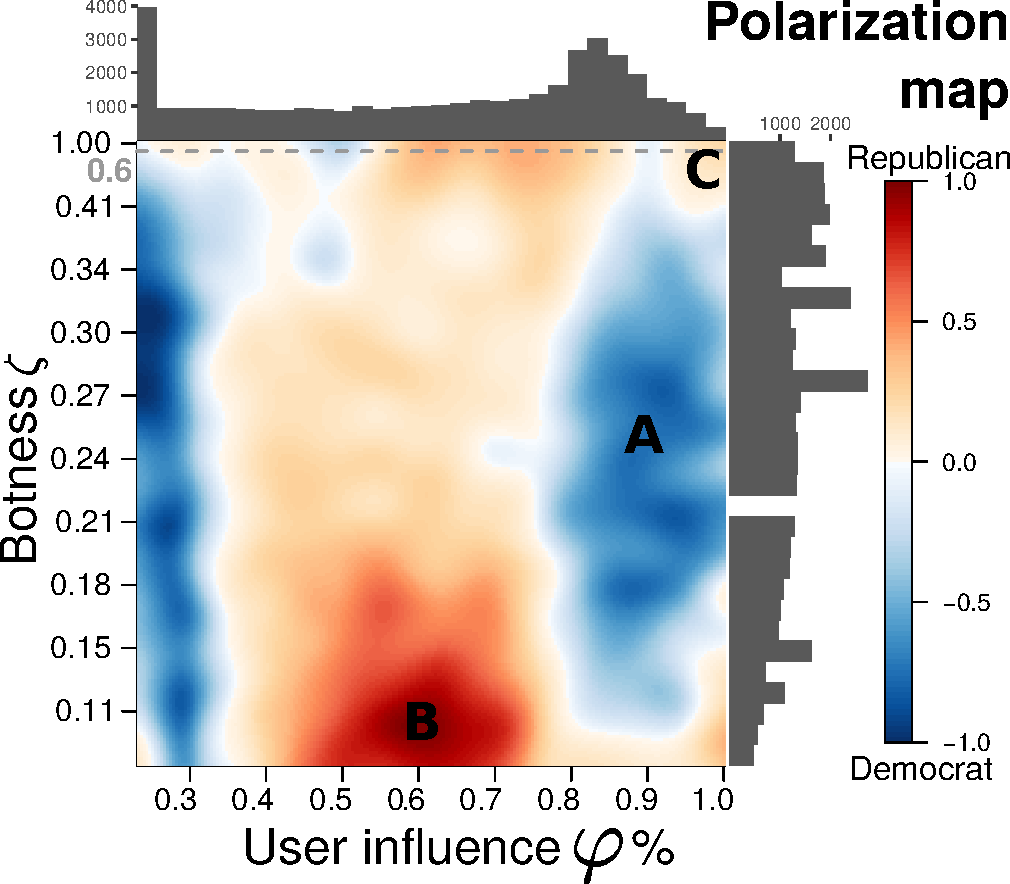
\includegraphics[width=0.47\textwidth]{influence-botscore-polarization-2d-map}

	\caption{ 
		Political polarization by user influence $\varphi(u) \%$ (x-axis) and bot score $\zeta$ (y-axis).
%		The x-axis shows the percentile of user influence, from 0 being the least influential to 1 being the most influential.
%		The y-axis shows the bot score. 
		% (see the distribution of bot score density in Fig.~\ref{subfig:botscore-density}).
		The gray dashed horizontal line shows the threshold of 0.6 above which a user is considered a bot.
		The color in the map shows political polarization: areas colored in bright blue (red) are areas where the Democrats (Republicans) have considerably higher density than Republicans (Democrats).
		%: it is the ratio of the density of Democrat users to the density of Republican users.
%		Areas where the density of Republicans is considerably higher than the density of Democrats are colored bright red (and similarly for bright blue).
		Areas where the two populations have similar densities are colored white.
		Three areas of interest are shown by the letter \textbf{A}, \textbf{B} and \textbf{C}.
	}
	\label{fig:polarization-map}
%	\captionmoveup
\end{figure}